
\subsection{Breif}
\paragraph{What is Neural Networks?}
Artificial neural networks are one of the main tools used in machine learning. As the “neural” part of their name suggests, they are brain-inspired systems which are intended to replicate the way that we humans learn. Neural networks consist of input and output layers, as well as (in most cases) a hidden layer consisting of units that transform the input into something that the output layer can use. They are excellent tools for finding patterns which are far too complex or numerous for a human programmer to extract and teach the machine to recognize.

\paragraph{}
While neural networks (also called “perceptrons”) have been around since the 1940s, it is only in the last several decades where they have become a major part of artificial intelligence. This is due to the arrival of a technique called “backpropagation,” which allows networks to adjust their hidden layers of neurons in situations where the outcome doesn’t match what the creator is hoping for — like a network designed to recognize dogs, which misidentifies a cat, for example.

\paragraph{}
Another important advance has been the arrival of deep learning neural networks, in which different layers of a multilayer network extract different features until it can recognize what it is looking for.

\subsection{Basics of Neural Networks.}
\paragraph a basic idea of how a deep learning neural network learns, imagine a factory line. After the raw materials (the data set) are input, they are then passed down the conveyer belt, with each subsequent stop or layer extracting a different set of high-level features. If the network is intended to recognize an object, the first layer might analyze the brightness of its pixels. see figure 1.2
	
\begin{figure}{l}
	\centering
	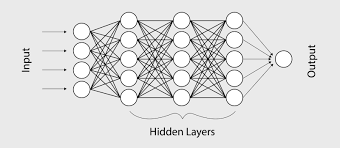
\includegraphics[width=1.0\textwidth]{CH1-introduction/sec3_neural_networks/nn.png}
	\caption{example of neural networks}
\end{figure} 

\paragraph{}
The next layer could then identify any edges in the image, based on lines of similar pixels. After this, another layer may recognize textures and shapes, and so on. By the time the fourth or fifth layer is reached, the deep learning net will have created complex feature detectors. It can figure out that certain image elements (such as a pair of eyes, a nose, and a mouth) are commonly found together.
\paragraph{}
Once this is done, the researchers who have trained the network can give labels to the output, and then use backpropagation to correct any mistakes which have been made. After a while, the network can carry out its own classification tasks without needing humans to help every time.
\paragraph{}
Beyond this, there are different types of learning, such as supervised or unsupervised learning or reinforcement learning, in which the network learns for itself by trying to maximize its score

\subsection{Why Neural networks are important? }
\paragraph{}
ANNs (Artificial Neural Networks) have some key advantages that make them most suitable for certain problems and situations:
\begin{enumerate}
	\item ANNs have the ability to learn and model non-linear and complex relationships, which is really important because in real-life, many of the relationships between inputs and outputs are non-linear as well as complex.
	\item ANNs can generalize ,After learning from the initial inputs and their relationships, it can infer unseen relationships on unseen data as well,thus making the model generalize and predict on unseen data.
	\item  Unlike many other prediction techniques, ANN does not impose any restrictions on the input variables (like how they should be distributed). Additionally, many studies have shown that ANNs can better model heteroskedasticity i.e. data with high volatility and non-constant variance, given its ability to learn hidden relationships in the data without imposing any fixed relationships in the data. 
	
\end{enumerate}
\subsection{Types of neural network }
\paragraph{}
There are multiple types of neural network, each of which come with their own specific use cases and levels of complexity.
\newline
\subsubsection{\textbf feedforward neural network}

\paragraph{}The most basic type of neural net is something called a feedforward neural network, in which information travels in only one direction from input to output.
\paragraph{}neural network layers are independent of each other; hence, a specific layer can have an arbitrary number of nodes. Typically, the number of hidden nodes must be greater than the number of input nodes. When the neural network is used as a function approximation, the network will generally have one input and one output node. When the neural network is used as a classifier, the input and output nodes will match the input features and output classes.
\paragraph{}A neural network must have at least one hidden layer but can have as many as necessary. The bias nodes are always set equal to one. In analogy, the bias nodes are similar to the offset in linear regression 
i.e. y = mx+b. How does one select the proper number of nodes and hidden number of layers? This is the best part: there are really no rules! The modeler is free to use his or her best judgment on solving a specific problem. Experience has shown that there are best practices such as selecting an adequate number of hidden layers, activation functions, and training methods
see figure (1.3).
\begin{figure}
	\centering
	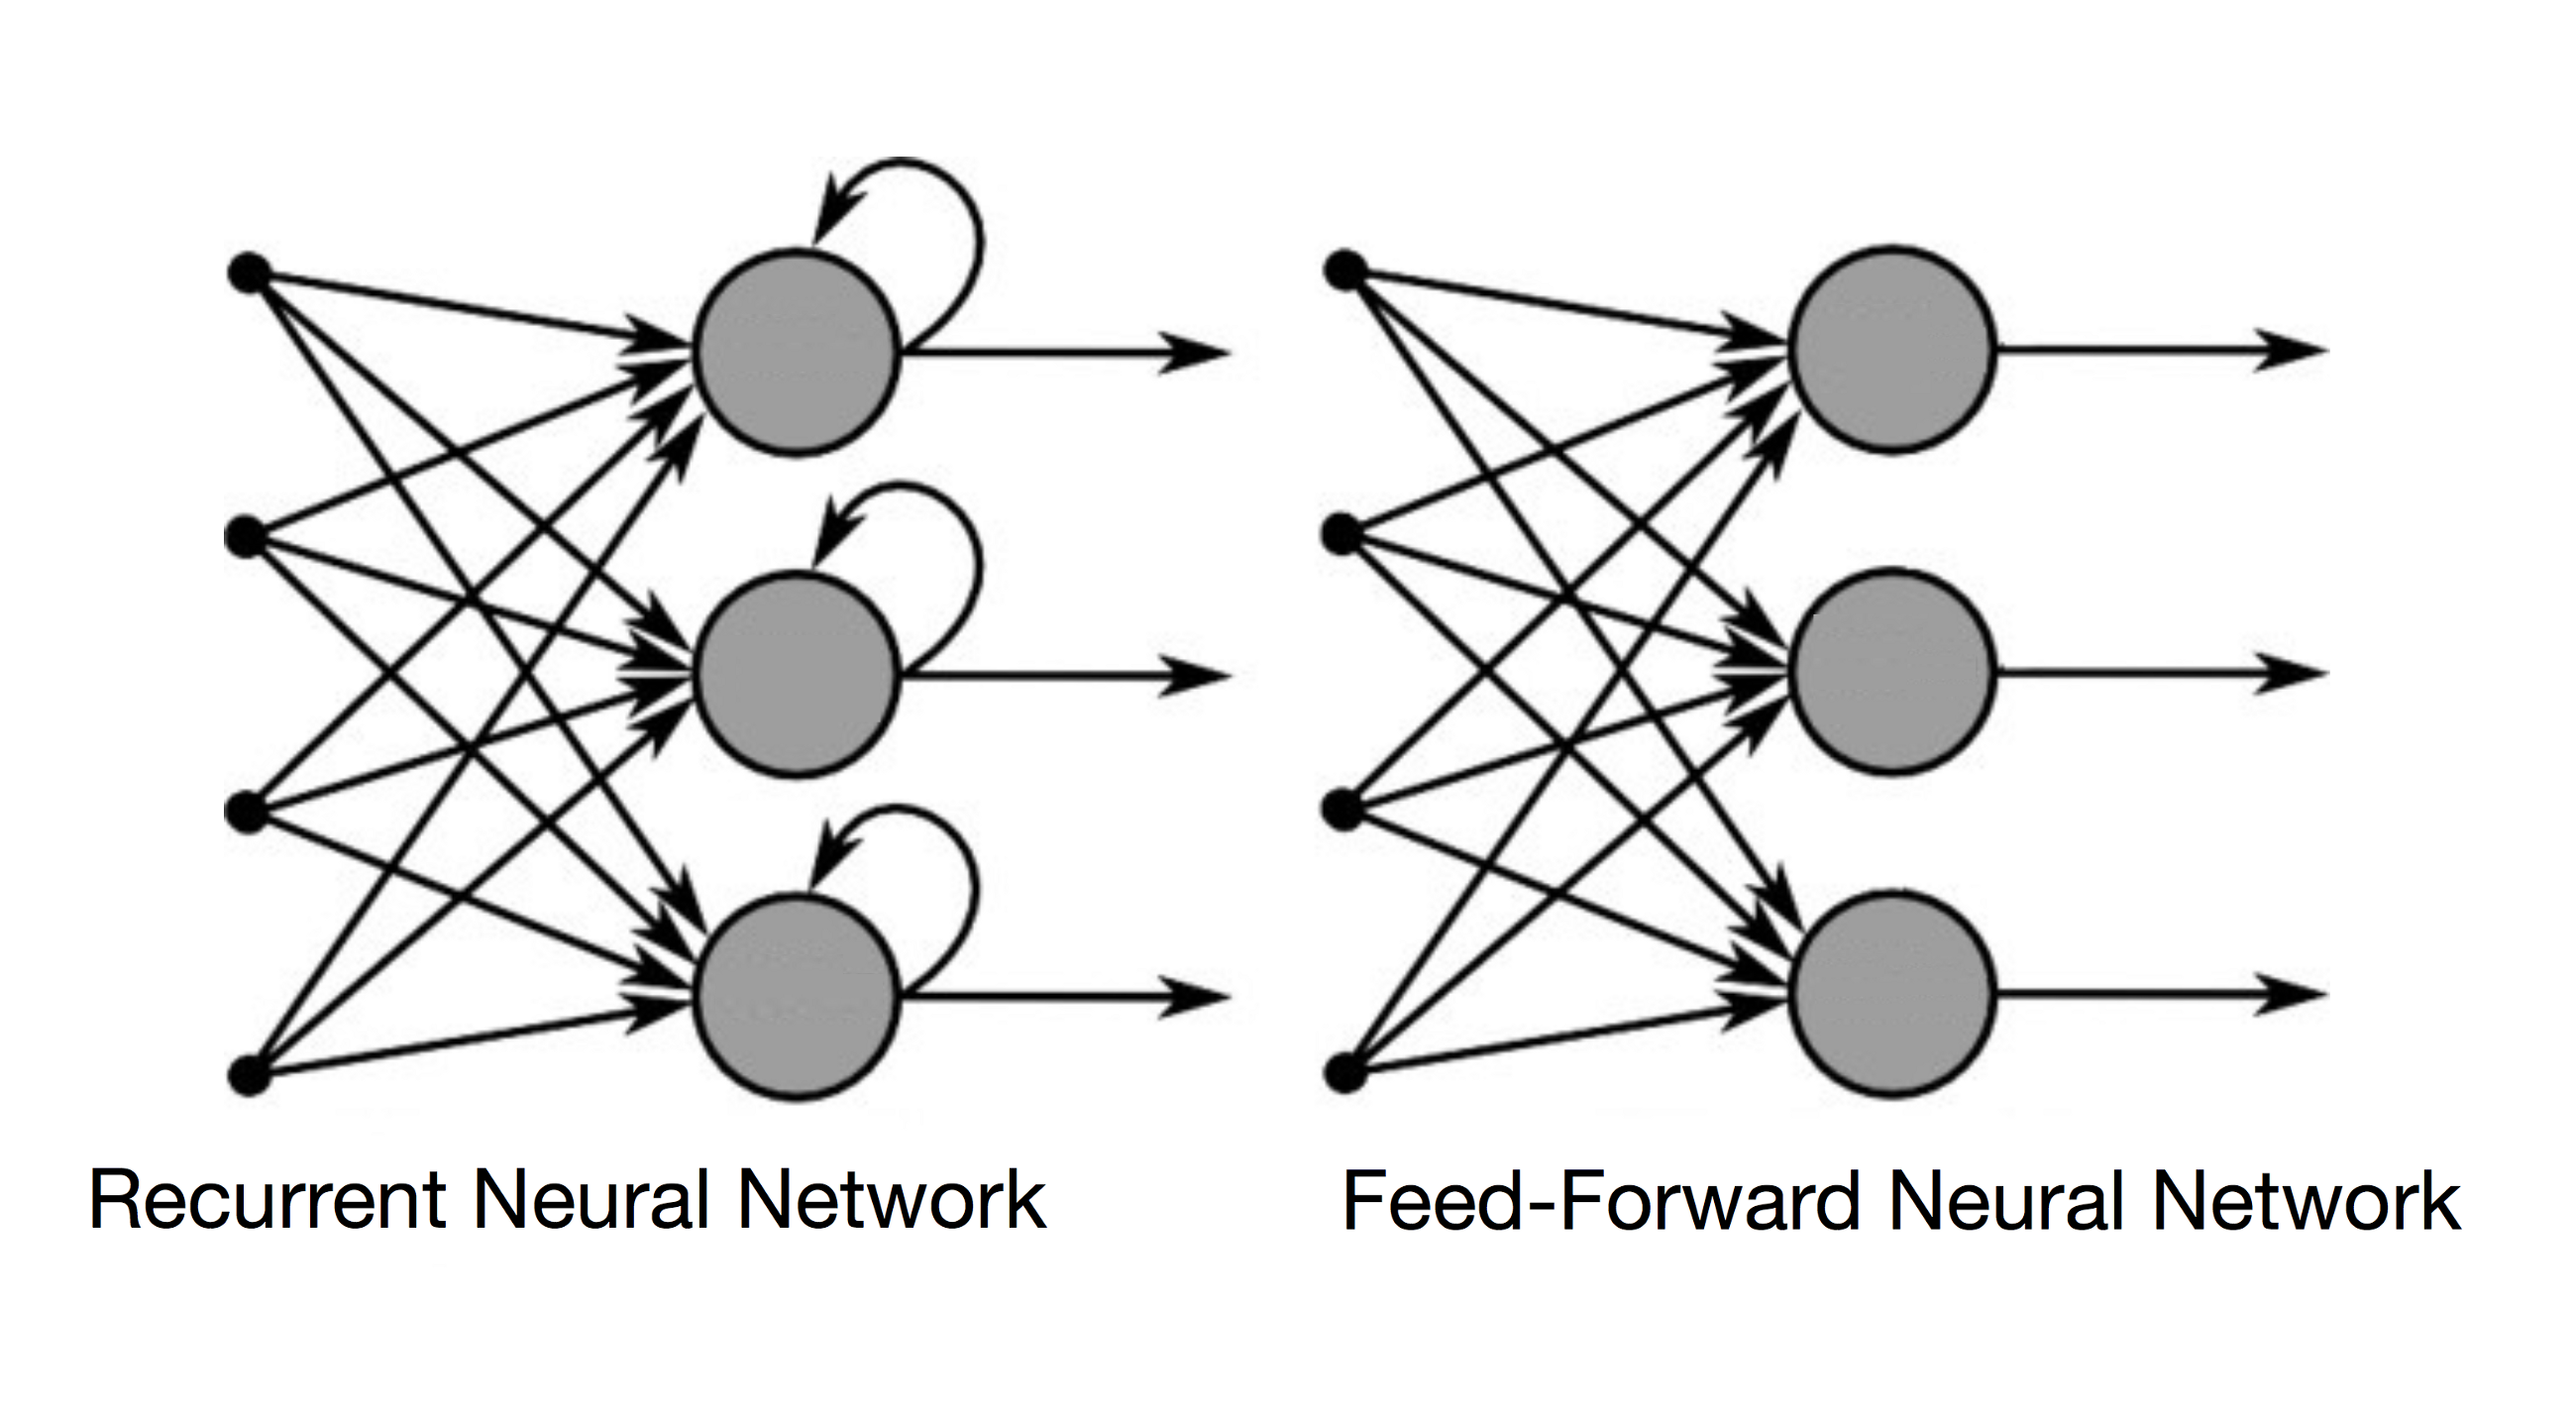
\includegraphics[width=0.7\textwidth]{rf.png}
	\caption{Structure of Feedforward and Recurrent Neural networks.}
\end{figure}
\subsubsection{Recurrent Neural Network
}
\paragraph{}
A recurrent neural network (RNN) is a type of artificial neural network commonly used in speech recognition and natural language processing (NLP). RNNs are designed to recognize a data's sequential characteristics and use patterns to predict the next likely scenario. see figure (1.3) 
\subsubsection{Convolutional Neural Network
}
\paragraph{}
A convolutional neural network (CNN) is a type of artificial neural network used in image recognition and processing that is specifically designed to process pixel data.

\paragraph{}
CNNs are powerful image processing, artificial intelligence (AI) that use deep learning to perform both generative and descriptive tasks, often using machine vison that includes image and video recognition, along with recommender systems and natural language processing (NLP).
\paragraph{}
A convolution is the simple application of a filter to an input that results in an activation. Repeated application of the same filter to an input results in a map of activations called a feature map, indicating the locations and strength of a detected feature in an input, such as an image.
\subsection{How Neural network is  useful for Facial Emotion Detection}
\paragraph{}
Analysis and recognition of human facial expressions
from images and video form the basis for understanding
image content at a higher semantic level. Expression
recognition forms the core task of intelligent systems
based on human-computer interaction (HCI). So the main task here is "understanding images and video content", this is the core concept of neural networks train over a lot of samples to learn then we can apply the concept of generalization on it by testing it using unseen data and check the output. 
as I mention above  there are different types of learning, here we  use Supervised learning as we feed the neural network with labeled data so we lead the training process.
\paragraph{}
So according to our application, we choose to build our model using the convolutional neural networks (CNN).
\paragraph{}
Traditional neural networks are not ideal for image processing and must be fed images in reduced-resolution pieces. CNN has their “neurons” arranged more like those of the frontal lobe, the area responsible for processing visual stimuli in humans and other animals. The layers of neurons are arranged in such a way as to cover the entire visual field avoiding the piecemeal image processing problem of traditional neural networks.

\subsection{A Gentle Introduction to Convolutional Neural Network Layers }   
The innovation of convolutional neural networks is the ability to automatically learn a large number of filters in parallel specific to a training dataset under the constraints of a specific predictive modeling problem, such as image classification. The result is highly specific features that can be detected anywhere on input images.
\paragraph{}
A CNN uses a system much like a multilayer perceptron that has been designed for reduced processing requirements. The layers of a CNN consist of an input layer, an output layer and a hidden layer that includes multiple convolutional layers, pooling layers, fully connected layers and normalization layers. The removal of limitations and increase in efficiency for image processing results in a system that is far more effective, simpler to trains limited for image processing and natural language processing.
\subsubsection{Convolutional Layer}
\paragraph{}
Convolution is the first layer to extract features from an input image. Convolution preserves the relationship between pixels by learning image features using small squares of input data. It is a mathematical operation that takes two inputs such as image matrix and a filter or kernal multiply them and get another matrix as a result which  is called the feature map.
\begin{figure}
	\centering
	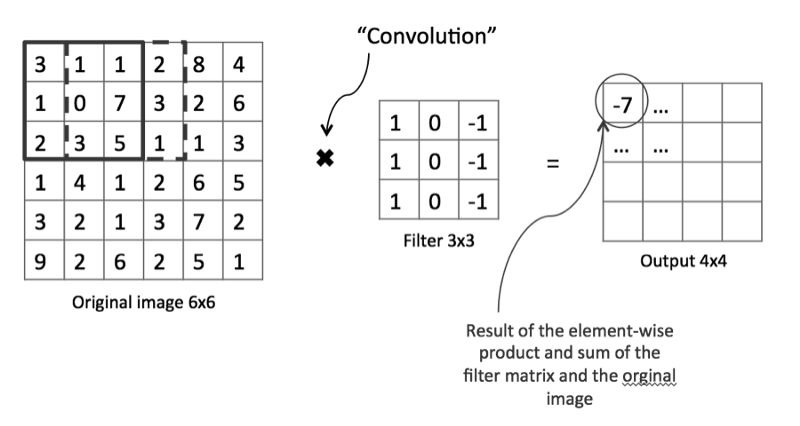
\includegraphics[width=0.7\textwidth]{conv_layer.png}
	\caption{example of Convolutional layer.}
\end{figure}
\paragraph{}
Convolution of an image with different filters can perform operations such as edge detection, blur and sharpen by applying filters. The below example shows various convolution image after applying different types of filters (Kernels).
\subsubsection{Stride}
Stride is the number of pixels shifts over the input matrix. When the stride is 1 then we move the filters to 1 pixel at a time. When the stride is 2 then we move the filters to 2 pixels at a time and so on. The below figure shows convolution would work with a stride of 2.
\begin{figure}
	\centering
	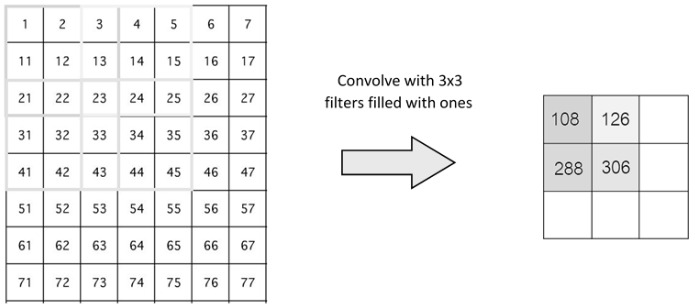
\includegraphics[width=0.7\textwidth]{stride.jpg}
	\caption{example of stride.}
\end{figure}
\subsubsection{Padding}
Sometimes filter does not fit perfectly fit the input image. We have two options:

Pad the picture with zeros (zero-padding) so that it fits Drop the part of the image where the filter did not fit. This is called valid padding which keeps only valid part of the image.
\subsubsection{Relu}
\paragraph{}
ReLU stands for Rectified Linear Unit for a non-linear operation. The output is $f\left(x\right) = max\left( (0,x\right)$.
% <-- \begin{figure}
% <-- 	\centering
% <-- 	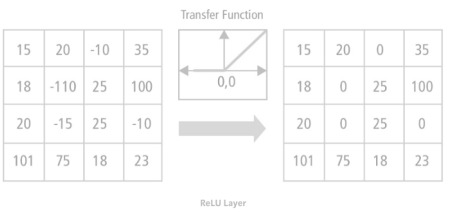
\includegraphics[width=0.7\textwidth]{relu.jpg}
% <-- 	\caption{example of Relu function}
% <-- \end{figure} 
\paragraph{}
Why ReLU is important : ReLU’s purpose is to introduce non-linearity in our ConvNet. Since, the real world data would want our ConvNet to learn would be non-negative linear values.
\paragraph{}
There are other non linear functions such as tanh or sigmoid can also be used instead of ReLU. Most of the data scientists uses ReLU since performance wise ReLU is better than other two.
\subsubsection{Pooling Layer}
\paragraph{}
Pooling layers section would reduce the number of parameters when the images are too large. Spatial pooling also called subsampling or downsampling which reduces the dimensionality of each map but retains the important information. Spatial pooling can be of different types:
\begin{enumerate}
	\item Max Pooling
	\item Average Pooling
	\item Sum Pooling
\end{enumerate}
\paragraph{}
Max pooling take the largest element from the rectified feature map. Taking the largest element could also take the average pooling. Sum of all elements in the feature map call as sum pooling.
\begin{figure}
	\centering
	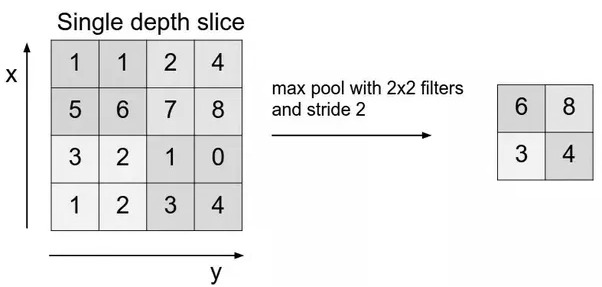
\includegraphics[width=0.7\textwidth]{pooling_layer.jpg}
	\caption{example of pooling layer}
\end{figure}
\subsubsection{Fully connected Layer}
The layer we call as FC layer, we flattened our matrix into vector and feed it into a fully connected layer like neural network.





